\documentclass[11pt,a4paper,oneside]{report}             % Single-side
%\documentclass[11pt,a4paper,twoside,openright]{report}  % Duplex

%\PassOptionsToPackage{chapternumber=Huordinal}{magyar.ldf}
\usepackage{t1enc}
\usepackage[utf8]{inputenc}
\usepackage{amsmath}
\usepackage{amssymb}
\usepackage{enumerate}
\usepackage[thmmarks]{ntheorem}
\usepackage{graphics}
\usepackage{epsfig}
\usepackage{listings}
\usepackage{color}
%\usepackage{fancyhdr}
\usepackage{lastpage}
\usepackage{anysize}
\usepackage[magyar]{babel}
\usepackage{sectsty}
\usepackage{setspace}  % Ettol a tablazatok, abrak, labjegyzetek maradnak 1-es sorkozzel!
\usepackage[hang]{caption}
\usepackage{hyperref}

%--------------------------------------------------------------------------------------
% Main variables
%--------------------------------------------------------------------------------------
\newcommand{\vikszerzo}{Hajnal Máté}
\newcommand{\vikkonzulens}{Albert István}
\newcommand{\vikcim}{Gantt diagramm alkalmazás HTML5-tel}
\newcommand{\viktanszek}{Automatizálási és Alkalmazott Informatikai Tankszék}
\newcommand{\vikdoktipus}{Önálló Labóratorium}
\newcommand{\vikdepartmentr}{Hajnal Máté}

%--------------------------------------------------------------------------------------
% Page layout setup
%--------------------------------------------------------------------------------------
% we need to redefine the pagestyle plain
% another possibility is to use the body of this command without \fancypagestyle
% and use \pagestyle{fancy} but in that case the special pages
% (like the ToC, the References, and the Chapter pages)remain in plane style

\pagestyle{plain}
%\setlength{\parindent}{0pt} % áttekinthetõbb, angol nyelvû dokumentumokban jellemzõ
%\setlength{\parskip}{8pt plus 3pt minus 3pt} % áttekinthetõbb, angol nyelvû dokumentumokban jellemzõ
\setlength{\parindent}{12pt} % magyar nyelvû dokumentumokban jellemzõ
\setlength{\parskip}{0pt}    % magyar nyelvû dokumentumokban jellemzõ

\marginsize{35mm}{25mm}{15mm}{15mm} % anysize package
\setcounter{secnumdepth}{0}
\sectionfont{\large\upshape\bfseries}
\setcounter{secnumdepth}{2}
\singlespacing
\frenchspacing

%--------------------------------------------------------------------------------------
%	Setup hyperref package
%--------------------------------------------------------------------------------------
\hypersetup{
    bookmarks=true,            % show bookmarks bar?
    unicode=false,             % non-Latin characters in Acrobat’s bookmarks
    pdftitle={\vikcim},        % title
    pdfauthor={\vikszerzo},    % author
    pdfsubject={\vikdoktipus}, % subject of the document
    pdfcreator={\vikszerzo},   % creator of the document
    pdfproducer={Producer},    % producer of the document
    pdfkeywords={keywords},    % list of keywords
    pdfnewwindow=true,         % links in new window
    colorlinks=true,           % false: boxed links; true: colored links
    linkcolor=black,           % color of internal links
    citecolor=black,           % color of links to bibliography
    filecolor=black,           % color of file links
    urlcolor=black             % color of external links
}

%--------------------------------------------------------------------------------------
% Set up listings
%--------------------------------------------------------------------------------------
\lstset{
	basicstyle=\scriptsize\ttfamily, % print whole listing small
	keywordstyle=\color{black}\bfseries\underbar, % underlined bold black keywords
	identifierstyle=, 					% nothing happens
	commentstyle=\color{white}, % white comments
	stringstyle=\scriptsize\sffamily, 			% typewriter type for strings
	showstringspaces=false,     % no special string spaces
	aboveskip=3pt,
	belowskip=3pt,
	columns=fixed,
	backgroundcolor=\color{lightgray},
} 		
\def\lstlistingname{lista}	

%--------------------------------------------------------------------------------------
%	Some new commands and declarations
%--------------------------------------------------------------------------------------
\newcommand{\code}[1]{{\upshape\ttfamily\scriptsize\indent #1}}

% define references
\newcommand{\figref}[1]{\ref{fig:#1}.}
\renewcommand{\eqref}[1]{(\ref{eq:#1})}
\newcommand{\listref}[1]{\ref{listing:#1}.}
\newcommand{\sectref}[1]{\ref{sect:#1}}
\newcommand{\tabref}[1]{\ref{tab:#1}.}

\DeclareMathOperator*{\argmax}{arg\,max}
%\DeclareMathOperator*[1]{\floor}{arg\,max}
\DeclareMathOperator{\sign}{sgn}
\DeclareMathOperator{\rot}{rot}
\definecolor{lightgray}{rgb}{0.95,0.95,0.95}

\author{\vikszerzo}
\title{\viktitle}
\includeonly{
	guideline,%
	project,%
	titlepage,%
	declaration,%
	abstract,%
	introduction,%
	chapter1,%
	chapter2,%
	chapter3,%
	acknowledgement,%
	appendices,%
}
%--------------------------------------------------------------------------------------
%	Setup captions
%--------------------------------------------------------------------------------------
\captionsetup[figure]{
%labelsep=none,
%font={footnotesize,it},
%justification=justified,
width=.75\textwidth,
aboveskip=10pt}

\renewcommand{\captionlabelfont}{\small\bf}
\renewcommand{\captionfont}{\footnotesize\it}

%--------------------------------------------------------------------------------------
% Table of contents and the main text
%--------------------------------------------------------------------------------------
\begin{document}
\pagenumbering{arabic}
\onehalfspacing
%--------------------------------------------------------------------------------------
%	The title page
%--------------------------------------------------------------------------------------
\begin{titlepage}
\begin{center}
\includegraphics[width=150mm,keepaspectratio]{figures/eiffel_tower.png}\\
\vspace{0.3cm}
\textbf{Budapesti Mûszaki és Gazdaságtudományi Egyetem}\\
\textmd{Villamosmérnöki és Informatikai Kar}\\
\textmd{\viktanszek}\\[5cm]

\vspace{0.4cm}
{\huge \bfseries \vikcim}\\[0.8cm]
\vspace{0.5cm}
\textsc{\Large \vikdoktipus}\\[4cm]

\begin{tabular}{cc}
 \makebox[7cm]{\emph{Készítette}} & \makebox[7cm]{\emph{Konzulens}} \\
 \makebox[7cm]{\vikszerzo} & \makebox[7cm]{\vikkonzulens}
\end{tabular}

\vfill
{\large \today}
\end{center}
\end{titlepage}



\tableofcontents\vfill
%----------------------------------------------------------------------------
\chapter*{Bevezető}\addcontentsline{toc}{chapter}{Bevezetõ}
%----------------------------------------------------------------------------

\hspace{2mm} Az elmúlt néhány évben hatalmas fejlődés volt a nem-triviális kvantumszámítógépek készítése terén.
Rengeteg start-up dolgozik a technológia üzleti alapokra helyezésével, a NIST standardizálja az új "post-quantum" titkostítási rendszerét, és ipari nagyóriások, mint a Google és a Microsoft, tesznek lépéseket manapság, hogy megvédjék rendszereiket a jövőben lehetséges rosszindulatú kvantumtámadásoktól.
Ezek a széleskörben alkalmazható kvantumszámítógépek már a mi életünk alatt is megszülethetnek.

\indent Az első elektromos számítógépek - a Mark I, Clossus, és ENIAC - drágák, nehezen használhatóak és lassú gépek voltak, elsősorban csak a kormánynak dolgozó kódfeltörőknek és a hadifegyver-készítőknek voltak csak hasznára.
Hasonlóan ezekhez a gépekhez az első kvantumszámítógépek is drágák, lassúak lesznek és alkalmazásuk csak a hagyományos titkosítási rendszerek feltörésére, mint az RSA, valamint a fizaki szimulációk futtatására fog kiterjedni.

\indent Szerencsére számunkra, az idővel a klasszikus számítógépek hardvere olcsóbbá és gyorsabbá vált, és a modern operációs rendszerek által biztosított hardver-absztrakciók, virtuális memória, és időosztás  a számítógéper könnyebben használhatóvá, biztonságosabbá és gyorsabbá tették a mindennap embere számára.

\indent A kérdés tehát, hogy az új kvantumszámítógépeink milyen architektúrát igényelnek és, hogy a milyen operációs rendszer is fog ezeken a gépeken futni?
Ebben a dokumentumban felfedezhetjük a \textit{kvantum operációs rendszer} lehetőségeit, kérdéseit azokkal a részleges válaszokkal, amik egy ilyen új típusú operációs rendszer tervezéséhez kellenek.
\begin{itemize}
\item Milyen új absztrakciók szükségesek egy kvantum operációs rendszer programozásához?
\item A kvantum számítógépek ereje, hogyan tudja megnövelni a klasszikus rendszerek teljesítményét?
\item Hogyan nézne ki egy elosztott kvantum számítógép? És milyen új funkcionalitást tud egy ilyen gép biztosítani?
\end{itemize}

\indent Ez a dokumentum szükségesen (és szégyenszerűen) spekulatív:
Még túlságosan korai egy pontos leírást adni egy csak 20, 50 vagy 100 év múlva létező hardverre...
Egyelőre annyit tehetünk, hogy a meglévő kvantumszámlálási modelleket ráillesztjük egy ilyen széleskörű kvantumszámítógépre, hogy elképzeljük milyen lesz majd az, amikor a jövőben megvalósul.

\indent Az olvasó meglehetősen szkeptikusan nézheti most ezt a dokumentumot, mint egy összefoglalója a negatív eredményeknek: a jelenlegi ismereteink szerint, nincs túl sok olyan dolog most, amit a felhasználó egy kvantumszámítógéppel tud csak megcsinálni és egy hagyományos gyors klasszikus számítógéppel nem.
A célünk hát szimplán, hogy tegyünk egy megjegyzést a kvantum számítógépeknél arra a logikus kérdésre, hogy milyen lenne, ha ott lenne mindannyiunk asztalán egy ilyen mágikus kvantumszámítógép?

\indent A dokumentumban három lehetséges architektúrát vázolunk fel, haladva a legkevésbé merésztől a legmerészebb elképzelésig:
Először is a kvantum FPGA-król ejtünk szót, utána a kvantum x86-os számítógépekről, és végül a kvantum elosztott rendszerekről.
Mindegyiknél fogjuk tárgyalni, hogy a gép hogyan kezelné a legalapvetőbb feladatokat, mint a fuzz tesztelés, CPU ütemezés és párhuzamos programozás.
Beszélünk arról is, hogy az egyes architektúrák hogyan felelnek meg a rendszerszintű kihívásoknal.

%----------------------------------------------------------------------------
\chapter{C-RAN koncepció}\label{sect:CranConcept}
%----------------------------------------------------------------------------
\section{Mi is az a C-RAN?}

\hspace{2mm}\cite{RecentCRANProg} \cite{Architecture} \cite{ImplementationIssues} \cite{BenefitsFujitsu} \cite{BenefitsEricsson} \cite{WirelessFull}  \cite{FutureCarrier} \cite{ImplementingGPP} \cite{NokiaSingle} \cite{TechOverview}   Az amerikai származású gépész mérnök Henry Gantt-tól származik a nevét is örző Gannt diagramm forma. Ma már a projektmenedzsment mindennapjait kiséri végig ez a feladatok ütemezését vizuálisan megragadó eszköz. Maga a diagram egy elfektetett oszlopdiagramhoz hasonlít, amelyen követhetjük a projekthez tartozó egyes feladatok elvégzésének egy ütemezését. \cite{GanttChart} Két nagyobb megjelenítendő részből áll, egy a feladatokat listázza, egy pedig a naptárszerű rész mely az elvégzési ütemtervet mutatja. 

\begin{figure}[!ht]
\centering
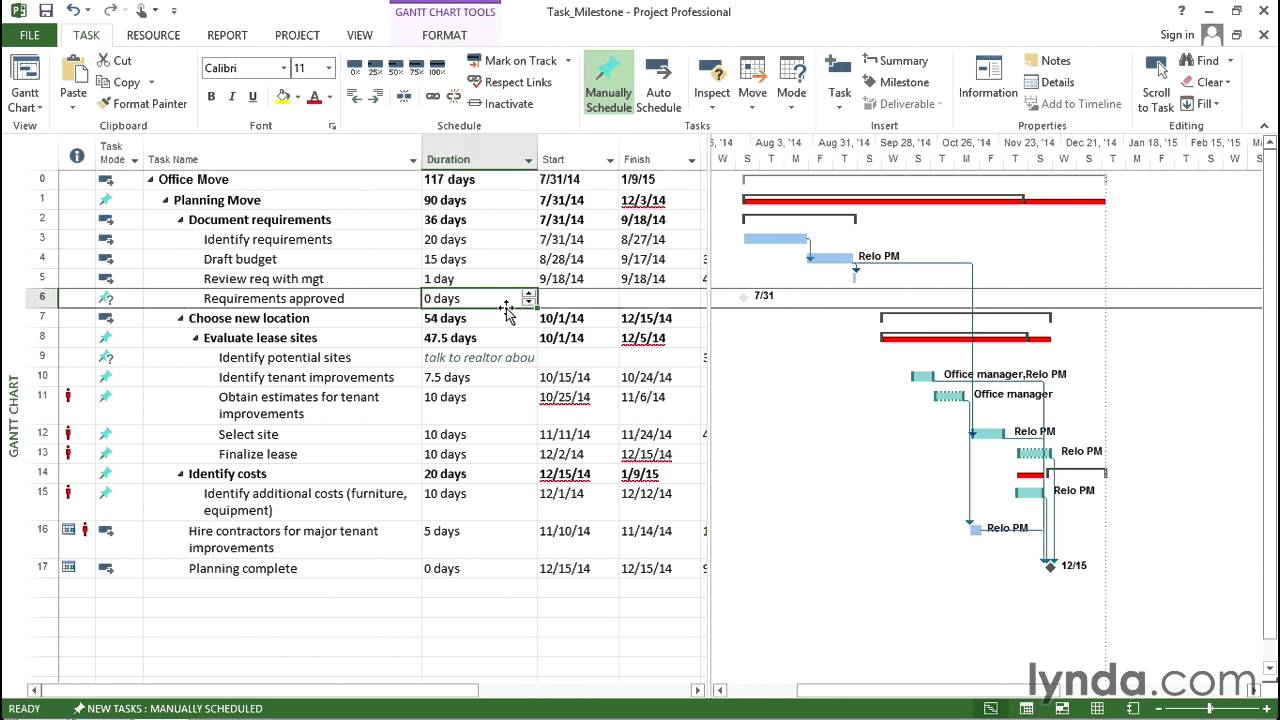
\includegraphics[width=\textwidth, keepaspectratio]{figures/msproject.jpg}
\caption{Microsoft Project 2016 Gantt program kinézete} 
\label{fig:MSProject}
\end{figure} 

A Microsoft Project által megvalósított Gantt vastag kliens alkalmazásra mutat példát a \figref{MSProject}-es ábra. Az ábrán megfigyelhetők a taskok legfontosabb tulajdonságai. Minden tasknál beállíthatjuk, hogy mennyi ideig fog tartani és, hogy milyen függöségei vannak, ezután a task kezdési és végzési idejét az alkalmazás az ütemezés függvényében állítja majd be. Láthatjuk, hogy nem csak feladatok vannak, hanem azoknak egy öszefoglalója, summaryje is melyek alá több feladat tartozhat. Fontos, hogy ez a summary nem egy külön task, hanem azoknak egy gyűjtője, az elvégzési időtartama is az alatta lévő taskok összege. Még érdemes azt is megemlíteni, hogy a program a taskok egymásutániságát nyílakkal is szemlélteti a jobb érthetőség és vizualizáció érdekében. \cite{RecentCRANProg}

A Microsoft Project ellenpontjaként több projekt próbálta vékonykliensen is megvalósítani az alkalmazást egy webes applikáció keretében, ilyen például a GanttPro, melyben a Microsoft Project legtöbb funkciója implementálásra került. A programba a \figref{GanttPro} ábra nyújt betekintést, feladatom a félév során egy ehhez hasonló alkalmazás alapjainak lefektetése volt.\cite{GanttPro}

\begin{figure}[!ht]
\centering
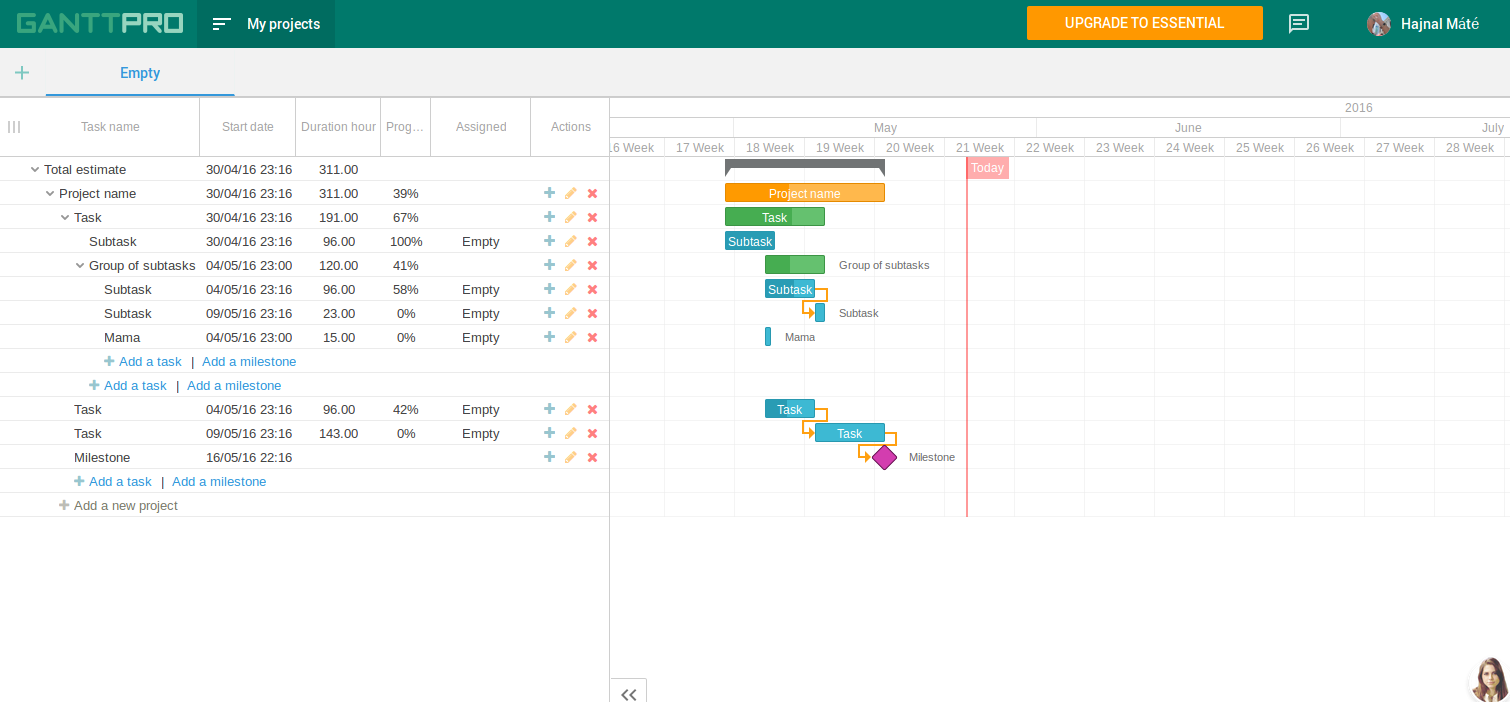
\includegraphics[width=\textwidth, keepaspectratio]{figures/ganntpro.png}
\caption{A GanttPro webes alkalmazás} 
\label{fig:GanttPro}
\end{figure} 

%----------------------------------------------------------------------------
\section{C-RAN Tulajdonságai}
\hspace{2mm} \indent Az irodalomkutatás során az első algoritmus amibe belebotlottam a Kritikus út módszer (Critical Path Method CPM). Maga a Gantt diagram inkább a megjelenítésre fókuszál, a benne lefutó algoritmusokról semmit nem mond, így ezek után az algoritmusok után kellett keresnem a félévben.  Fontos leszögeznem, hogy nincs jelenleg nem NP-nehéz tökéletes megoldása a feladatnak, így a jelenleg legelterjedtebb megoldások közül választottam. A CPM egy ilyen megoldás, mely ha előre ismerjük a feladatok végrehajtási idejét, azok erődorrásait és függőségeit, akkor segít kiszámolni a lehetséges kezdési és befejezési időpontokat. \cite{CPM}

\begin{figure}[!ht]
\centering
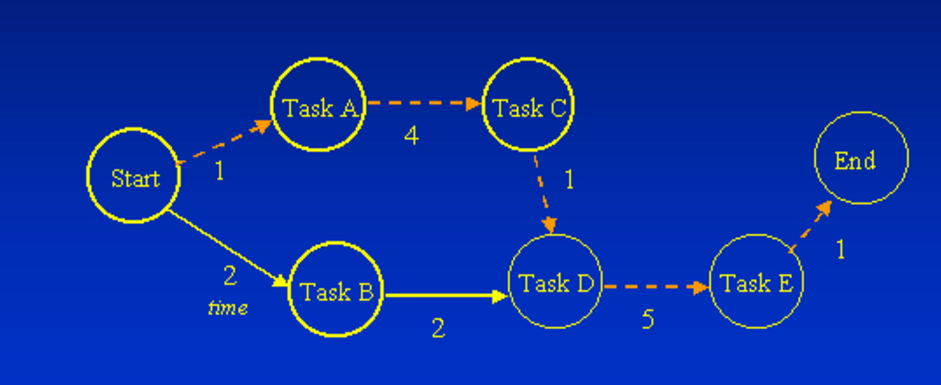
\includegraphics[width=\textwidth, keepaspectratio]{figures/cpm.png}
\caption{A Kritikus út módszerre példa} 
\label{fig:CPM}
\end{figure} 

A \figref{CPM}-es ábrán szemlélhetjük az algoritmus futását. A Start pontból indulunk és a Finish pontba szeretnénk eljutni. Az algoritmus először kiszámítja minden lehetséges útvonalra az úthosszt (ez 11 és 10), ami egy egszerű gráf algoritmust jelent, majd végül a leghosszabb útat választja, ez lesz a kritikus útvonal. Könnyen végig gondolható, hogy azért van ez így, mert a feladatok szempontjából ez az útvonal jelöli a legszűkebb keresztmetszetet, hiszen ennél hamarabb nem tudunk végezni a projekttel.

%----------------------------------------------------------------------------
\section{C-RAN Kihívásai}
\hspace{2mm}  \indent CPM-mel megtaláltuk a projektünk szempontjából legkritikusabb utat, így a végrehajtást ennek az útvonalnak a végigjárásával kell kezdenünk. Viszont a CPM  a projektben lévő többi feladat elvégzéséről nem mond semmit. Ehhez egy másik algoritmust találtam a Least Slack Time scheduling algoritmusát, azonbelül is a First verziót, mely magyarul úgy hangozhat, hogy "Legkisebb tartalékú először" algoritmus.\cite{LST} Az algoritmus lényege, hogy minden feladatnak ad egy prioritást az alapján, hogy mennyire "halogatható" (slack time) az adott feladat. A halogatási időhöz ki kell számolni minden feladatra a legkorábbi kezdési időpontot és a legkésőbbi végzési időpontot, a kettő különbsége a slack time. Ebből az előbbi a CPM algoritmusából már adódik, az utóbbit pedig úgy definiálhatjuk, mint az az időpont, amikor a feladatot legkésőbb végre kell hajtani, hogy ne legyen még csúszás a projektben. Ennek megkapásához egy újabb CPM algoritmust kell futtani úgy, hogy megfordítjuk a futás irányát, azaz a függőségeket és a kezdési időpontnak beállítjuk az utolsó feladat legkorábbi befejezési időpontját. 


%\listoffigures\addcontentsline{toc}{chapter}{Ábrák jegyzéke}
%\listoftables\addcontentsline{toc}{chapter}{Táblázatok jegyzéke}

\bibliography{mybib}
\addcontentsline{toc}{chapter}{Irodalomjegyzék}
\bibliographystyle{plain}

\label{page:last}
\end{document}
